\documentclass[tikz, class=beamer]{standalone}
\usetheme{metropolis}
\usepackage{braket}

\definecolor{star}{RGB}{236, 195, 91}
\definecolor{aqarius}{RGB}{71, 115, 255}
\definecolor{feascolor}{RGB}{121, 174, 144}
\definecolor{failcolor}{RGB}{216, 65, 65}
\definecolor{aqua}{RGB}{16, 34, 64}
\definecolor{sand}{RGB}{241, 237, 229}
\colorlet{xsand}{sand!50}

\setbeamercolor{normal text}{fg=aqua, bg=xsand}

\newcommand{\splitarrow}[8]{
    \pgfmathsetmacro{\pos}{#1}
    \pgfmathsetmacro{\width}{#2}
    \pgfmathsetmacro{\height}{#3}
    \pgfmathsetmacro{\prob}{#4}
    \pgfmathsetmacro{\aw}{#5}
    \pgfmathsetmacro{\saw}{#6}
    \pgfmathsetmacro{\rem}{(1 - \prob) * \height}
    \pgfdeclareverticalshading{myshading}{10cm}{
        color(0)=(failcolor!30);
        color(0.4cm)=(#8!30);
        color(1.8cm)=(#8!30)
    }
    \draw[xshift=\pos,thick, shading=myshading] (0, 0) -- ++(\width-\aw, 0) -- ++(\aw, -0.5*\prob*\height)
    -- ++(-\aw, -0.5*\prob*\height) arc (90:0:\aw) -- ++(0, -\rem+\aw-0.1) -- ++(-0.5 * \saw, -0.1) 
    -- ++(-0.5*\saw, 0.1) arc (0:90:0.1) -- (0, -\height) -- cycle;
    \node[xshift=\pos,rotate=-90] at (0.5 * \width - 0.25 * \aw , -0.5 * \height) {#7};
    \node[xshift=\pos,color=failcolor!50!black] at (\width-0.5 * \saw , -\height -0.5)
    {\small failed};
}

\begin{document}

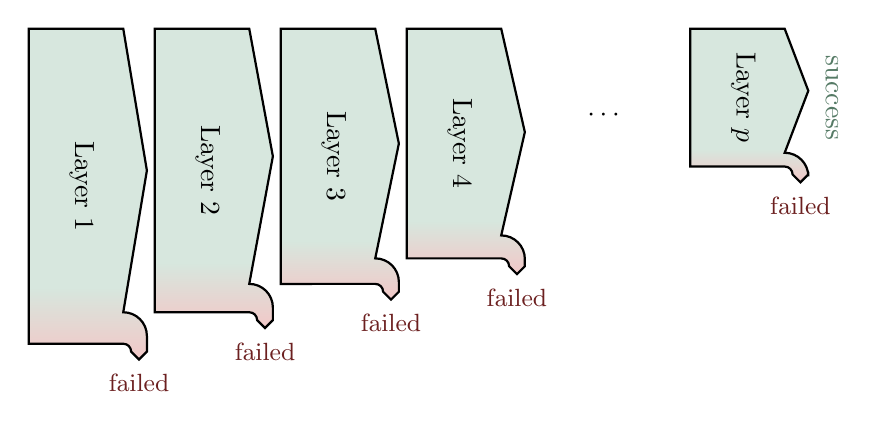
\begin{tikzpicture}[
        full/.style={thick,fill=start!30,draw=black!80},
        feas/.style={thick,fill=feascolor,draw=black!80},
        arrow/.style={very thick,fill=green,draw=black!70}
    ]
    % \splitarrow{0cm}{1.5}{5}{0.8}{0.3}{0.3}{State initialization}{feascolor}
    \splitarrow{1.6cm}{1.5}{0.8 * 5}{0.9}{0.3}{0.2}{Layer 1}{feascolor}
    \splitarrow{3.2cm}{1.5}{0.9 * 0.8 * 5}{0.9}{0.3}{0.2}{Layer 2}{feascolor}
    \splitarrow{4.8cm}{1.5}{0.9 * 0.9 * 0.8 * 5}{0.9}{0.3}{0.2}{Layer
    3}{feascolor}
    \splitarrow{6.4cm}{1.5}{0.9 * 3.24}{0.9}{0.3}{0.2}{Layer 4}{feascolor}
    \node at (8.9cm, -1.1cm) {$\cdots$};
    \splitarrow{10cm}{1.5}{0.6 * 0.9 * 3.24}{0.9}{0.3}{0.2}{Layer $p$}{feascolor}
    % \splitarrow{1.02cm}{1}{2}{0.9}{0.2}{0.2}
    % \splitarrow{2.04cm}{1}{1.8}{0.9}{0.2}{0.2}
    % \splitarrow{2.04cm}{1}{1.8}{0.9}{0.2}{0.2}

    \node[color=feascolor!70!black, rotate=-90] at (11.8cm, -0.875cm) {success};
\end{tikzpicture}

\end{document}
